\documentclass[9pt,twoside]{pnas-new}

\articletype{Collective behavior}
\templatetype{pnasmathematics}

% no "DRAFT" watermark, no placeholder footer, no affiliation box in the margin
% (it overlaps the full-width text); the affiliation goes in the dates line instead
\setboolean{displaywatermark}{false}
\makeatletter
\def\PNAS@dropfoot[#1]#2{}
\patchcmd{\ps@firststyle}{\fancyfoot[L]}{\PNAS@dropfoot[L]}{}{\PackageError{report}{footer patch failed}{}}
% no line numbers (the template draws a fixed column in the header, not aligned with the text)
\apptocmd{\ps@firststyle}{\fancyhead{}}{}{\PackageError{report}{header patch failed}{}}
\patchcmd{\ps@firststyle}{\thepage of}{\thepage\ of}{}{\PackageError{report}{page patch failed}{}}
\def\PNAS@linecountsecpageLO{}\def\PNAS@linecountsecpageRO{}
\def\PNAS@linecountsecpageLE{}\def\PNAS@linecountsecpageRE{}
\fancyfoot{}
\fancyfoot[RO,LE]{\footerfont\textbf{\thepage\ of \pageref*{LastPage}}}
\additionalelement{}
\makeatother

\raggedbottom
\urlstyle{same} % URLs in the text font
\AtBeginDocument{\hypersetup{urlcolor=black}}
\DefineJournalException{Journal of the Royal Society Interface}{J. R. Soc. Interface}
\DefineJournalException{Royal Society Open Science}{R. Soc. Open Sci.}
\DefineJournalException{Scientific Reports}{Sci. Rep.}
\begin{document}

\title{From hunter to shepherd: does the optimal alignment of a fish school depend on the agent that perturbs it?}

\author{Mathieu Bonnet, Loup Benois and Alexandre Peret}


\leadauthor{Bonnet}

\begin{abstract}
Fish schools under attack are thought to benefit from being close to the transition between
disordered and ordered motion. Klamser and Romanczuk showed with a predator--prey model that schools
are indeed caught least there. According to them, the reason is mainly the looser structure of the school, not a better
collective response. This project asks whether this optimum still holds when the school faces a
different agent: first a more realistic predator, then a shepherd that tries to move the school
instead of catching prey. In this first report, models of collective motion, predation and
shepherding are reviewed. The model of Klamser and Romanczuk is reimplemented in Python and validated
against the original code, and the minimum of the capture rate at the transition is reproduced (about 13\% fewer captures).
The next reports will test whether this minimum stays at the transition for an improved predator,
in 2D and 3D, and whether the transition also helps a shepherd.
\end{abstract}

\dates{Faculty of Computer and Information Science, University of Ljubljana. First report, November 13, 2026}

\maketitle
\thispagestyle{firststyle}
\ifthenelse{\boolean{shortarticle}}{\ifthenelse{\boolean{singlecolumn}}{\abscontentformatted}{\abscontent}}{}

\section*{Introduction}

When a predator attacks a fish school, the prey do not react independently. They turn, split and
regroup together, so the predator has to deal with a moving target that keeps changing shape. One
explanation of how such groups process information is the criticality hypothesis: living groups would
operate close to a phase transition, where their response to perturbations is largest~\cite{mora2011,munoz2018}.
For moving groups, the transition of interest is the one between a disordered swarm and an ordered,
polarized school. It appears in models of self-propelled particles when alignment becomes stronger
than noise~\cite{vicsek1995,couzin2002}.

Klamser and Romanczuk~\cite{klamser2021} tested this hypothesis with a model in which a single
predator attacks a school of 400 prey. The capture rate is lowest near the order--disorder
transition, but not for the reason the hypothesis gives. They compared the attacked school with an
identical school that does not flee. The fraction of prey saved by fleeing keeps increasing with
alignment and has no peak at the transition. The advantage of the critical school therefore comes
from its spatial structure, which is looser, and not from a better collective response. They also
let the alignment strength evolve. Each prey survives better by aligning more, so the population ends
up far in the ordered phase: the transition is best for the group, but evolution does not keep it
there.

These results are obtained with one specific predator. It swims twice as fast as the prey, heads for
a weighted center of the prey in front of it, and always follows the same rule. Real predators choose
the direction of their attack~\cite{bartashevich2024}, combine tactics such as splitting a school
before isolating a prey~\cite{demsar2015}, and get confused when many prey move around
them~\cite{olson2013}. Would a different predator change which alignment protects a school best? This
does not seem to have been tested. The opposite question is open as well. The high
responsiveness at criticality does not explain the low capture rate, but it could be useful for an
agent that wants to steer a school without breaking it, like a sheepdog with a flock~\cite{strombom2014}
or a group of robots with fish~\cite{vanhavermaet2024}. Such agents could lead groups away from dangers
or along a given path~\cite{vanhavermaet2023,vanhavermaet2024}.

The question is therefore whether the benefit of being near the order--disorder transition depends
on the agent that perturbs the school. The project has three steps: reproduce the model of Klamser and Romanczuk,
improve its predator and move to three dimensions, then turn the predator into a shepherd that moves
the school without breaking it. This first report
reviews existing models, presents the reimplementation and the reproduced result, and describes the
next steps.

\section*{Related work}

\paragraph*{Collective motion and criticality}
Vicsek et al.~\cite{vicsek1995} showed that self-propelled particles that align with their neighbors
have a phase transition. Below a critical noise level the group moves in a common direction; above
it, the motion is disordered. Couzin et al.~\cite{couzin2002} added short-range repulsion and
long-range attraction, and obtained the main collective states seen in nature: swarm, milling and
parallel motion. Statistical models fitted to real data, from neurons to bird flocks, seem to be close
to a critical point. This led to the hypothesis that biological systems are tuned to
criticality~\cite{mora2011}. Mu\~noz~\cite{munoz2018} reviews the arguments for it, mainly a maximal
sensitivity to stimuli and a large range of possible behaviors, and notes that the evidence is still
indirect.

\paragraph*{Predator--prey models}
Klamser and Romanczuk~\cite{klamser2021} combine a Vicsek-like school with a pursuing predator, and
evolve the alignment strength of the prey with an evolutionary algorithm. Their predator is
deliberately simple. Other studies focus on the predator itself. Dem\v{s}ar et al.~\cite{demsar2015}
evolved composite hunting tactics with a genetic algorithm, for example splitting a school before
catching an isolated prey. The dispersing tactic was the best one only when the predator could be confused by the prey.
Olson et al.~\cite{olson2013} showed that predator confusion alone is enough for swarming to evolve in
prey. Bartashevich et al.~\cite{bartashevich2024}, from the same group as Klamser, filmed striped
marlin attacking sardine schools. The ``fountain'' escape of the school depended on the direction of
the attack, and an agent-based model reproduced it.

\paragraph*{Shepherding}
Steering a group is the opposite task: the agent has to move the group without breaking it.
Str\"ombom et al.~\cite{strombom2014} proposed a single shepherd that collects the agents when they
are too spread out and drives them once they are grouped. Their model reproduces data from sheep and
sheepdogs. However, their sheep do not align with each other and stop when the dog is far away,
whereas fish swim all the time in an aligned school. Van Havermaet et
al. use several robots that surround the group, to keep a herd away from dangers~\cite{vanhavermaet2023}
or to guide simulated fish along a path~\cite{vanhavermaet2024}. Their method needs enough robots for the size of the group, so it is not
known whether a single agent could guide a fish school.

\section*{Methods}

\paragraph*{Model}
The model of Klamser and Romanczuk~\cite{klamser2021} and its C++ implementation are followed, with the
parameters of Table~\ref{tab:params}. Each of the $N = 400$ prey moves at a constant speed $v_0$. Its
heading $\mathbf{u}_i$ is a unit vector, which turns at each time step by
\begin{equation}
\delta\theta_i = \frac{1}{v_0}\left(\mathbf{F}_i \cdot \mathbf{u}_i^{\perp}\,\Delta t
+ \sqrt{2D\,\Delta t}\;\eta_i\right),
\label{eq:turn}
\end{equation}
where $\mathbf{u}_i^{\perp}$ is the heading rotated by $90^\circ$, $D$ is the angular noise and
$\eta_i$ is a standard Gaussian variable. Each prey interacts with its Voronoi neighbors
$\mathcal{N}_i$:
\begin{equation}
\mathbf{F}_i = \frac{1}{n_i}\sum_{j \in \mathcal{N}_i}\Big[\mu_d \tanh\!\big(m_d(r_{ij} - r_d)\big)\,
\hat{\mathbf{r}}_{ij} + \mu_{\mathrm{alg},i}\,v_0(\mathbf{u}_j - \mathbf{u}_i)\Big]
+ \mu_{\mathrm{flee}}\,\hat{\mathbf{e}}_{i}.
\label{eq:force}
\end{equation}
The first term keeps neighbors at a distance $r_d$ and the second one aligns the headings. The last
term pushes prey $i$ away from the predator, along the unit vector $\hat{\mathbf{e}}_i$, when the
predator is one of its neighbors. $n_i$ is a neighbor count (see Reimplementation). The individual
alignment strengths $\mu_{\mathrm{alg},i}$ are drawn around a mean value $\mu_{\mathrm{alg}}$.

The predator is twice as fast as the prey. It appears after an equilibration time $T_{\mathrm{eq}}$, at a distance of 4.5 from the school, from an almost random direction. It first heads for the center of the school. Once it is close, it heads for the prey in front of it,
weighted by their chance of being caught. A prey at a distance $d < r_{\mathrm{catch}}$ is caught
with probability $p = \gamma_a\,\Delta t\,(r_{\mathrm{catch}} - d)/(r_{\mathrm{catch}}\,n_c)$, where
$n_c$ is the number of prey in reach. Caught prey are removed.

\begin{table}[b]
\centering
\caption{Model parameters (Table S1 of~\cite{klamser2021}).}
\label{tab:params}
\begin{tabular}{llc}
\toprule
Parameter & Symbol & Value \\
\midrule
Number of prey & $N$ & 400 \\
Prey speed, preferred distance & $v_0$, $r_d$ & 1 \\
Angular noise & $D$ & 0.5 \\
Mean alignment strength (swept) & $\mu_{\mathrm{alg}}$ & 0--1.6 \\
Distance regulation strength, slope & $\mu_d$, $m_d$ & 2 \\
Flee strength & $\mu_{\mathrm{flee}}$ & 4 \\
Predator speed, pursuit strength & $v_p$, $\mu_p$ & 2 \\
Catch radius & $r_{\mathrm{catch}}$ & 3 \\
Attack rate & $\gamma_a$ & 1/3 \\
Equilibration, attack duration & $T_{\mathrm{eq}}$, $T_{\mathrm{simu}}$ & 200, 120 \\
Time step & $\Delta t$ & 0.02 \\
\bottomrule
\end{tabular}
\end{table}

\paragraph*{Reimplementation}
The model was rewritten in Python. Directions are stored as unit vectors, so the code can be
extended to three dimensions. Every run takes a seed and can be replayed, which is not possible with
the C++ code. When the code and the equations of the paper differ, the code is followed, because it
produced the published figures. The code divides the social force by about half the number of neighbors
($n_i$), and $n_c$ only counts the prey within $r_{\mathrm{catch}}$.

\paragraph*{Measures}
Two quantities are measured when the predator appears: the polarization
$\Phi = |\frac{1}{N}\sum_i \mathbf{u}_i|$, which is close to 0 for a disordered school and to 1 for
an aligned one, and the inter-individual distance (IID), the mean distance between all pairs of prey. The transition is placed at the maximum
of the susceptibility $\chi = \beta N(\langle\Phi^2\rangle - \langle\Phi\rangle^2)$, with
$\beta = 1/(D v_0)$. $\chi$ measures how much $\Phi$ varies between runs~\cite{klamser2021}. The capture
rate $\gamma_c$ is the number of captures per unit time. Each attack is repeated on a control school
that starts from the same state but does not flee. This gives a second capture rate
$\gamma_{c,\mathrm{NF}}$ and the escape ratio $R_{\mathrm{esc}} = 1 - \gamma_c/\gamma_{c,\mathrm{NF}}$.
The mean alignment strength $\mu_{\mathrm{alg}}$ is varied from 0 to 1.6 in steps of 0.1, with 40
runs per value. For validation, the C++ code is run with the same values.

\begin{figure}[!t]
\centering
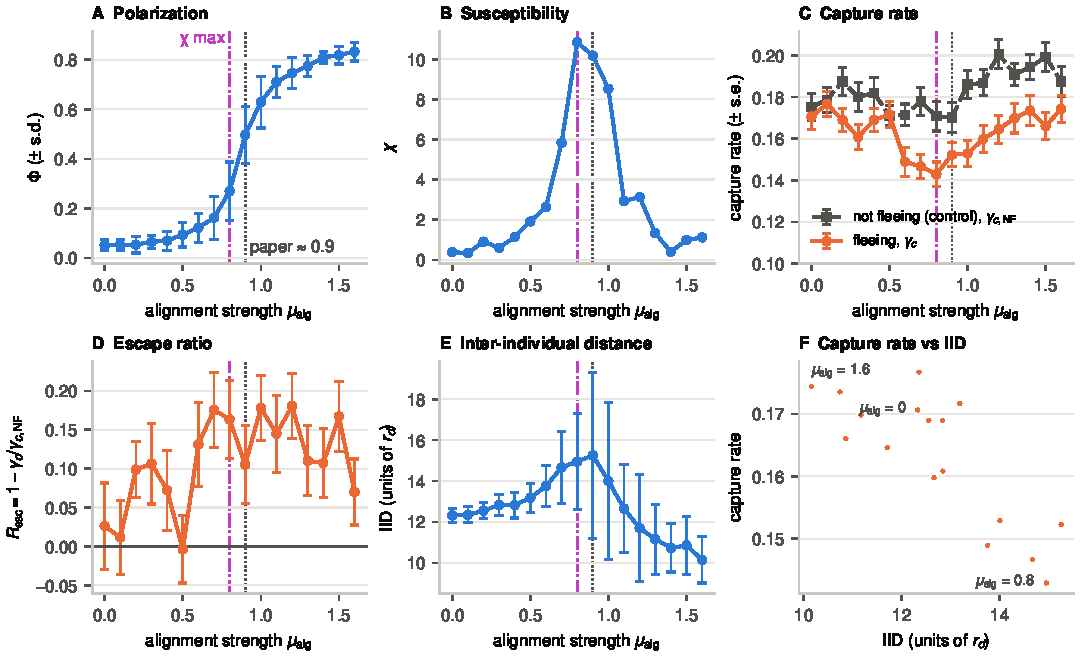
\includegraphics[width=\linewidth]{figures/sweep.pdf}
\caption{Order transition and predation against the alignment strength $\mu_{\mathrm{alg}}$
(parameters of Table~\ref{tab:params}, $D = 0.5$, 40 runs per point). (A) Polarization when the predator appears
($\pm$ s.d.). (B) Susceptibility. (C) Capture rate of the fleeing school $\gamma_c$ and of the
control school that does not flee $\gamma_{c,\mathrm{NF}}$ ($\pm$ s.e.; the y-axis does not start at 0). (D) Escape ratio
($\pm$ bootstrap s.e.). (E) Inter-individual distance when the predator appears ($\pm$ s.d.).
(F) Capture rate against the IID, one point per alignment strength ($R = -0.80$). Dash-dotted line: maximum
of $\chi$; dotted line: transition given by the paper.}
\label{fig:sweep}
\end{figure}


\paragraph*{Planned extensions}
Each extension only changes the agent that perturbs the school, and this agent only uses local
information. The prey rules, the sweep over $\mu_{\mathrm{alg}}$ and the control school stay the same,
so each new agent can be compared directly with the reproduced model (Table~\ref{tab:plan}).

For the second report, the predator will be improved in one way. One option is to choose the attack
direction relative to the heading of the school, as marlins do~\cite{bartashevich2024}. Another is to
head for the predicted position of the target instead of its current position. The question is
whether the capture-rate minimum stays at the transition. On the ordered side, where the dip comes from the structure of the
school, it should not move. On the disordered side, where it comes from fleeing, it may change. The model will then be moved to three
dimensions: headings become 3D unit vectors, the Voronoi neighbors are computed in 3D, and the
predator can also attack from below or above.

For the final report, the predator becomes a shepherd that moves the school to a target region. The
rules of Str\"ombom et al.~\cite{strombom2014} (collect the group when it is spread out, drive it
when it is grouped) will be adapted to fish. The main change is that the school keeps swimming and
aligning by itself, so the shepherd has to deflect a moving school, without making it flee and split.
The fraction of the school that reaches the target, the time needed and the number of groups the
school splits into will be measured as a function of alignment. One shepherd will also be compared
with the robot groups of Van Havermaet et al.~\cite{vanhavermaet2024}.

\begin{table}[t]
\centering
\caption{Plan of the project.}
\label{tab:plan}
\begin{tabular}{llll}
\toprule
Step & Agent & Main measure & Report \\
\midrule
1 & Original predator (2D) & Capture rate, escape ratio & Nov.~13, 2026 \\
2 & Improved predator (2D, then 3D) & Capture rate, escape ratio & Dec.~11, 2026 \\
3 & Shepherd & Fraction at target, time, splits & Jan.~8, 2027 \\
\bottomrule
\end{tabular}
\end{table}

\section*{Results}

\paragraph*{Validation against the original code}
C++ runs cannot be replayed, so the two codes can only agree on average. They do. The polarization
curves overlap, and the susceptibility peaks one step apart (0.9 for C++, 0.8 for Python). The
mean capture rate is also the same: 0.161 for the C++ code and 0.163 for the Python code. After a Bonferroni correction over the 17 values, no alignment strength shows a significant difference. The comparison figure is in the repository
(\texttt{report/figures/cpp\_comparison.pdf}). The main difference is that the dip of the C++ code is less deep on the
ordered side (7\% below the ordered phase, against 13\% for Python).

\paragraph*{Order and responsiveness}
When the alignment strength increases, the school goes from a disordered swarm, where prey head in all
directions ($\Phi \approx 0$), to a polarized school (Fig.~\ref{fig:sweep}A). The polarization rises
fastest and varies most between runs around $\mu_{\mathrm{alg}} \approx 0.8$, where the susceptibility
peaks (Fig.~\ref{fig:sweep}B). The order--disorder transition is placed there, close to the
value of 0.9 given in the paper.

\paragraph*{Group optimum}
The predator catches the fewest prey at the transition (Fig.~\ref{fig:sweep}C). For $\mu_{\mathrm{alg}} = 0.8$--$1.0$, the capture rate is about 13\% lower than in the disordered
($0$--$0.2$) or the ordered ($1.4$--$1.6$) phase. Both differences are significant (Welch t-tests, $p < 10^{-4}$). It corresponds to the group optimum of Fig.~2C of the paper.

\paragraph*{Fleeing or structure}
A school can be caught less because it escapes better, or because its spatial arrangement makes it
harder to attack. The control school has the same structure but does not flee, so it separates the two
effects. On average, fleeing helps: the control school loses more prey, and the escape ratio is about
0.1. However, the escape ratio has no peak at the transition (Fig.~\ref{fig:sweep}D): it rises from
the disordered phase, then stays at about 0.1--0.2. On the ordered side, the control school is also caught least near
the transition, so on this side the dip comes mostly from the structure of the school. On the disordered side, the control school is only about 3--4\% lower at the transition (not significant), so on this side the dip comes mostly from fleeing. Near the transition the school is also the most spread out
(Fig.~\ref{fig:sweep}E). Across alignment strengths, the inter-individual distance is strongly
anticorrelated with the capture rate ($R = -0.80$, Fig.~\ref{fig:sweep}F), as in the paper
($R = -0.69$).

\section*{Discussion}

The first result of Klamser and Romanczuk~\cite{klamser2021} is reproduced: a school is caught least
near the order--disorder transition, and, as in the paper, the escape ratio has no peak there. On the ordered side, the dip comes mostly
from the structure of the school; on the disordered side, mostly from fleeing.

There are two differences from the paper, and one point to keep in mind. First, the capture rates obtained here are
about 1.8 times higher than in Fig.~2C of the paper, but the curve has the same shape. The original
C++ code gives the same level as the Python code, so the difference is between the published code and the
published figure. It may come from the way captures are counted. Second, the escape ratio obtained here stops
increasing in the ordered phase, while that of the paper keeps increasing. With 40 runs per point
it is noisy, so its exact shape is uncertain. Finally, the link between inter-individual distance and
captures only holds across alignment strengths. At a fixed alignment strength, schools that are more
spread out are not caught less. Both quantities may simply depend on the alignment strength, without
one causing the other.

The reproduction uses a single noise level, $D = 0.5$. It also measures the school only once per run,
when the predator appears, which may be too early for schools near the transition to settle. The
evolution of alignment towards the ordered phase was not reproduced, as it is outside the scope of
this project.

These results give the baseline for the next steps. With 40 runs per point, the dip of the capture
rate is clearly detected, but the escape ratio is too noisy, so more runs may be needed for the new
predators. On the ordered side, the dip comes from the structure of the school, so it should stay for a
better predator. On the disordered side, it comes from fleeing, so a better predator may change it. For the shepherd, the transition could be useful for another reason: the school may respond strongly while staying in one group.

Code, data, figure scripts and the source of this report are available at\\
\url{https://github.com/mathieusharp/fish-school-predator-dynamics}.

\bibliography{references}

\end{document}
